\documentclass[11pt]{article}
\usepackage{amsmath, amssymb, amscd, amsthm, amsfonts}
\usepackage{graphicx}
\usepackage{hyperref}
\usepackage{natbib}
\usepackage{commath}
\usepackage{subfig}
\usepackage{float}
\usepackage{listings}
\oddsidemargin 0pt
\evensidemargin 0pt
\marginparwidth 40pt
\marginparsep 10pt
\topmargin -20pt
\headsep 10pt
\textheight 8.7in
\textwidth 6.65in
\linespread{2.0}

\title{Text Entry Interface Design And Evaluation: Literature Review}
\author{Tiankai Jiang\\20834939\\t57jiang@uwaterloo.ca}
\date{\today}

\newtheorem{theorem}{Theorem}
\newtheorem{lemma}[theorem]{Lemma}
\newtheorem{conjecture}[theorem]{Conjecture}

\providecommand{\keywords}[1]
{
  \small    
  \textbf{\textit{Keywords---}} #1
}

\newcommand{\rr}{\mathbb{R}}

\newcommand{\al}{\alpha}
\DeclareMathOperator{\conv}{conv}
\DeclareMathOperator{\aff}{aff}

\makeatletter
\setlength{\@fptop}{0pt}
\makeatother

\begin{document}

\maketitle

\begin{abstract}
This thesis analyzed 40 papers about text entry interface design and performance evaluation. And it aims to serve as a guideline and reference for researchers who want to conduct experiment in this field. The paper mainly focuses on methods to improve text entry user experience for physical keyboard and touch screen keyboard on mobile devices, and evaluation design details.
\end{abstract}

\keywords{text entry, usability evaluation, design principle, touch screen keyboard, physical keyboard}

\section{Introduction}\label{section-introduction}
Keyboard is one of the most important text entry methods. The origin of the keyboard can be traced back to the beginning of the 17th century in Europe. In 1868, an American inventor Christopher Latham Sholes got the patent and franchise of typewriter. Later, the prototype of modern keyboard layout(QWERTY) was developed. Beginning from 1950s, keyboards were massively used in computers. And since smartphones came out in the early 21st century, keyboards were migrated to smartphones in both physical form and a virtual touch screen form. Currently, there are more than 10 billion mobile devices(smartphones and tablets) in use worldwide and keyboard still serves as a primary input method. With the wide spread of keyboard and the extension of keyboard usage scenario, e.g. on smart TV, on smart watch, for the physically challenged, while driving, etc. the variation and improvement of the conventional keyboard on mobile devices is required to improve the performance and applicability.

40 papers related to text entry (mostly keyboard) design and evaluation were analyzed in this paper and the paper aims to answer the following questions:
\begin{itemize}
    \item What aspects could be considered to improve the user experience of the keyboard?
    \item What aspects could be considered to evaluate a keyboard?
    % \item What aspects could be considered to improve the accuracy of the evaluation of the keyboard performance?
\end{itemize}

\section{Methods to Improve Text Entry User Experience}\label{section-improvement}
User experience is related to the potential typing speed, the error rate on the keyboard, the mental workload while typing and the occupied area of the keyboard on the screen, etc. Several aspects were mentioned in the reviewed papers to improve text entry user experience: 
\begin{itemize}
    \item Visual improvement, e.g. making more space for content display.
    \item Feedback improvement, e.g. adding physical or voice feedback.
    \item Performance improvement, e.g. increasing typing speed and lowering error rate.
    \item Workload improvement, e.g. decreasing users' mental workload.
\end{itemize}
% \begin{itemize}
%     \item Hardware modification
%     \item Adding physical feedback to touch screen keyboard
%     \item Touch screen keyboard layout modification
%     \item Keyboard decoding algorithm improvement
% \end{itemize}
% The difference between layout modification and input form modification on touch screen keyboard is that the former still preserves the pressing action for the keyboard and only changes the keyboard layout or size of keys, etc. However, the latter only preserves the objective of the keyboard: text entry, but it can be done in a way of swiping or gestures, etc.
\subsection{Physical Keyboard Modification}
Although the number of mobile phones with physical keyboard has been decreasing sharply in recent years, qwerty phones still remain the preference for a minority of people and companies like BlackBerry still produce qwerty smart phones. Also, mobile devices with physical keyboard is an essenial for some people with disabilities. 

In the early days, mobile devices are not as portable as it is today. So their keyboard is relatively larger. \citet{10.1145/985921.986082} proposed a specialized keyboard, which compressed the 4-line characters and numbers in conventional keyboards into one line and used modifier keys and multitap to achieve character selection.
\begin{figure}[H]
  \centering
  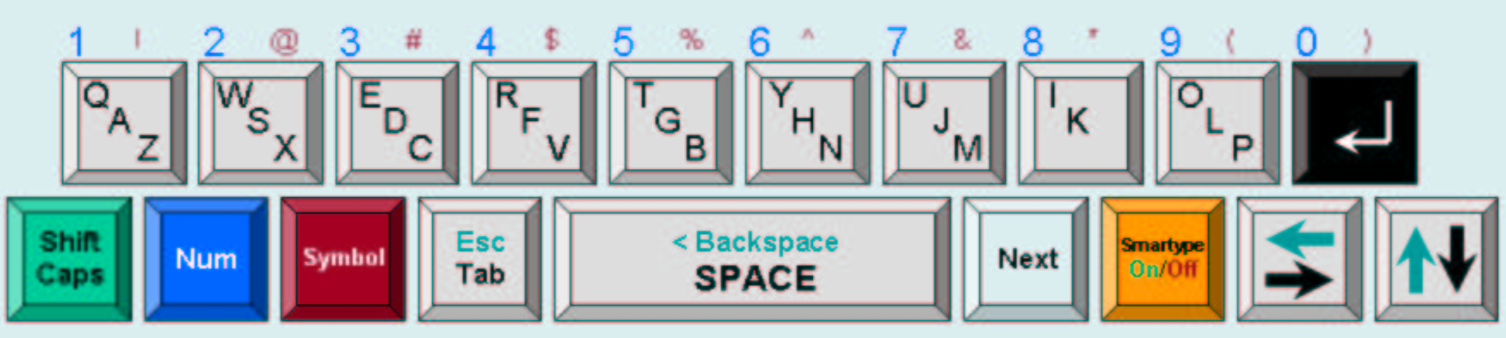
\includegraphics[width=0.8\textwidth]{ReducedQWERTYKeyboard.png}
  \caption{The reduced qwerty keyboard from \citep{10.1145/985921.986082}}
  \label{fig:reducedKeyboard}
\end{figure}

This design was motivated in two aspects, that the reduced keyboard only takes up 15\% to 25\% of the size of a normal keyboard and as we can see in Figure \ref{fig:reducedKeyboard}, each key is basically the compression of a normal keyboard in vertical direction so that the users could use their knowledge of the conventional keyboard. The experiment showed that after an average of 4.75 hours practice, participants could achieve half (10.4wpm) of their normal typing speed (22.5wpm). Although this was not an improvement in speed, considering the reduction in size and comparisons with its previous similar experiments, this experiment achieved a reasonable keyboard performance and learnability. It may seem naive currently since we have touch screen and more accurate sensors so we can reduce the key size. This design did not modify the size of the key, therefore, it is useful under some special conditions, e.g. text input on a small device in factories where the operators have to wear thick gloves so accurate operation cannot be performed. 

One of the biggest drawbacks of physical keyboard on mobile devices is that it takes up a lot of space that potentially can be used to present more content. \citet{10.1145/1851600.1851630} presented RearType, a text input system that uses normal keyboard keys but locates at the back of a device, aiming to maximize the use of display for visual output. 
\begin{figure}[H]
\centering
\subfloat[Front\label{fig:rearTypeA}]{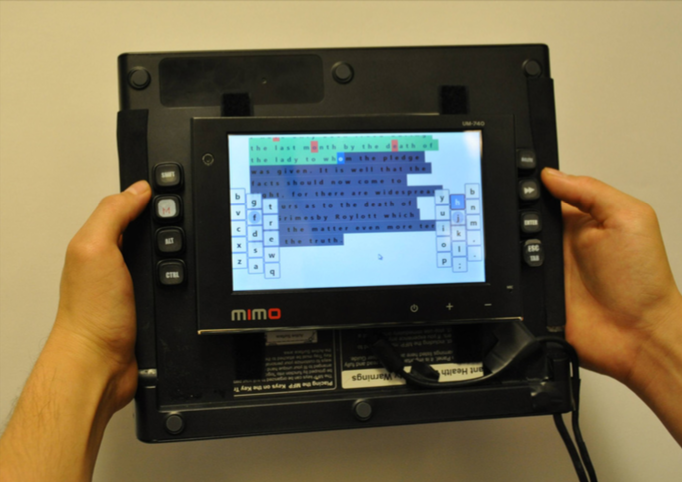
\includegraphics[width=0.5\textwidth]{RearType1.png}}\hfill
\subfloat[Back\label{fig:rearTypeB}] {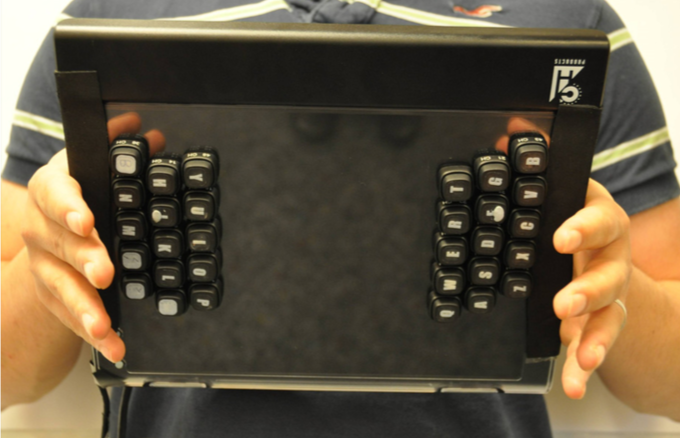
\includegraphics[width=0.5\textwidth]{RearType2.png}}\hfill
\caption{The RearType Keyboard from \citep{10.1145/1851600.1851630}} \label{fig:rearType}
\end{figure}
The RearType splited the QWERTY keyboard from the middle and rotated them by 90 degrees. So the keys have the same relative position as before, despite at the back, and the modifier keys locate at the front of the devices, within the approach of two thumbs (Figure \ref{fig:rearType}). So users can grab the devices using both hands while typing using all fingers. It is unreasonable to assume that users could touch type with this keyboard, so a semi-transparent floating widget on the screen was used to show which key was pressed.

The result showed that after 1 hour training, participants could achieve an average typing speed of 15 wpm, which was not statistically different to a touch screen keyboard. 

Similarly, \citet{10.1145/2212776.2223676} presented a physical QWERTY layout keyboard at the back of a mobile phone. Their design was more delicate than the previous one as it was for mobile phone only. The keyboard was placed at the top back of the mobile phone, splited in half as spatial cue for easy recognition of the keys' location. Users used their index fingers and/or middle fingers to type. The experiment found that after 40 minutes of exercise, participants could achieve a text entry rate of 15.3 wpm, with an error rate of 12.2\%. 

Both experiment proved that our knowledge about QWERTY layout can be transferred smoothly to the back of the device. This kind of design also seems crazy and unreasonable with little practical appeal. After all, the input speed did not increase with these designs. In the next section, a design similar to these keyboards was shown, but with a more modern approach.

\subsection{Touch screen at the back}
Generally, touch screen is more versatile than physical keyboards, for it can not only be used for typing, but also for gesture recognition and display. Since the existence of, no matter touch screen keyboard or physical keyboard, at the front of the device will reduce the area for displaying content, instead of adding a physical keyboard at the back, why not replace it with a touch screen at the back?

\begin{figure}[H]
  \centering
  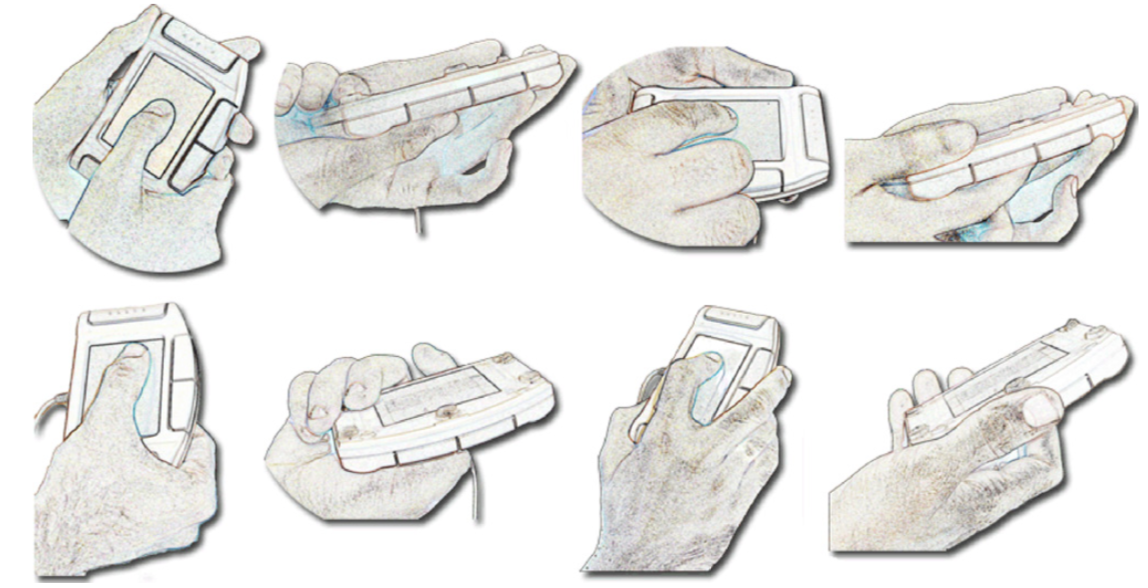
\includegraphics[width=0.8\textwidth]{HandPostureFrontBack.png}
  \caption{Touch screens on both sides of the device in \citep{10.1016/j.ijhcs.2008.03.004}}
  \label{fig:handposturefrontback}
\end{figure}

\citet{10.1016/j.ijhcs.2008.03.004} conducted experiments to check the feasibility of making gestures on the screen at the back of a mobile device. Their findings indicate that the index finger works well on the front and back of a device. And they showed that users could make letter-like gestures on the front and back of a device, and that the index finger on the front of the device performed best. Taken together, these studies indicate that device designs can go further to leverage a richer set of finger and thumb interactions. 

The experiment was taken in 2008, when the touch screen technology was still in its initial stage. The accuracy and the texture of the touchscreen were far from perfect.

Combining the result of this experiment and the previous two, we know that we are capable to both typing and making gestures at the back of a device. With the development of OLED display, the screen of a mobile phone can be extended to the back of the phone, such as Xiaomi Mix Alpha, and many high-end smartphones nowadays have two displays, at each side of the phone, with a much higher accuracy. The back type keyboard/gesture prototypes may not be used directly, but they serve as a good reference if a touch screen keyboard at the back of the device is needed. 

\subsection{Adding Physical Feedback to Touchscreen}

Generally, one of the drawbacks of touch screen is that there is no physical feedback when users make a press. So they do not know if they have truely touched the button, which may lead to extra key press.

\citet{10.1145/1357054.1357300} conducted an experiment to compare devices with a physical keyboard, a standard touchscreen and a touchscreen with tactile feedback. The result indicated that adding tacticle feedback to the touch screen could improve the performance of typing significantly. Later, they did the same experiment with a high specification actuator, which could roughly indicate the touch location. The result showed that the accuracy and speed improved even further. 

\citet{10.1145/1518701.1518750} surveyed the impact of tacticle feedback and audio feedback on the performance of text entry. The result indicated there was significant improvement on typing speed and error rate when using tacticle feedback and audio feedback. But there was no significant difference between using tacticle feedback and using audio feedback, and combining them together would not improve the result further. 

Both experiment indicated it was essential to add feedback to the touch screen. The application of physical feedback can be seen clearly throught the evolution of the iPhone. Since the first generation of iPhone, there was audio feedback when typing. From iPhone 6s, 3D touch was added, giving users a sense of "soft" and "heavy" when performing certain tasks. And later on iPhone XS, Apple replaced 3D touch with haptic touch, which not only showed different feedback strength, but also showing the feedback at the specific point where users pressed the screen using a two dimensional linear motor, making iPhone the one of the phones with the best typing experience.

\subsection{Touch Screen Keyboard Layout Modification}
One big advantage of software keyboard is that it can be modified to whatever layout we desire with little cost. The layout for the QWERTY keyboard was initially designed to avoid stucking in the typewriters. So, it does not necessarily ensure the performance on computer keyboard, let alone the performance on mobile devices. Therefore, a series of new keyboard layout were purposed in order to speed up typing on mobile devices.

\citet{10.1145/302979.302983} proposed a new keyboard layout for mobile devices (OPTI). Previous research summarized a 27$\times$27 table, showing the probability of the next character given the current character. The one more character, in addition to 26 letters, was space. The new layout was designed based on minimizing the path between every two characters according to that table.

\begin{figure}[H]
  \centering
  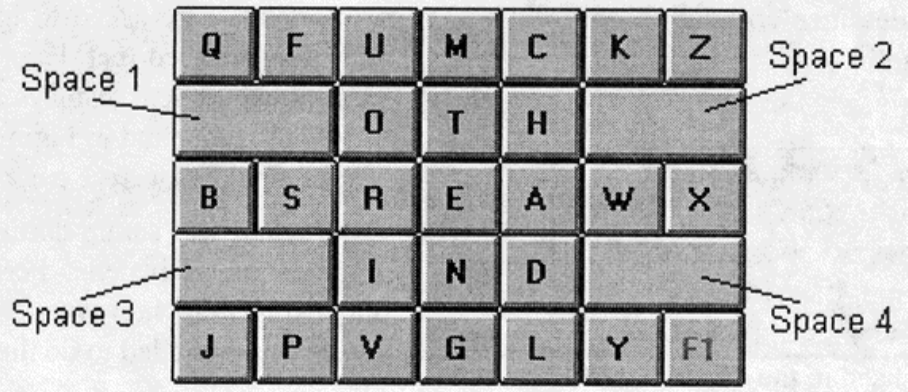
\includegraphics[width=0.8\textwidth]{Layout1999.png}
  \caption{New keyboard layout from \citep{10.1145/302979.302983}}
  \label{fig:layout1999}
\end{figure}

The layout was shown in Figure \ref{fig:layout1999}. The research assumed that users used one finger or a stylus pen for text entry. The result indicated that after 20 45-minutes training session, the text input speed increased from 17.0 wpm to 44.3 wpm. And some expert users achieved 58.2 wpm, which is 35\% faster than for the QWERTY layout. 

\citet{10.1145/1753326.1753367} mentioned that it was possible that some kind of layouts are more efficient than QWERTY layout, however, if the difference between QWERTY and the new layout were too large, it would be difficult and inconvenient to migrate from the conventinal layout to the new one. Hence, they proposed Quasi-Qwerty optimization. The overall performance would be increased and at the same time, the new layout was closed to the QWERTY layout, avoiding the problem mentioned above. 

\begin{figure}[H]
  \centering
  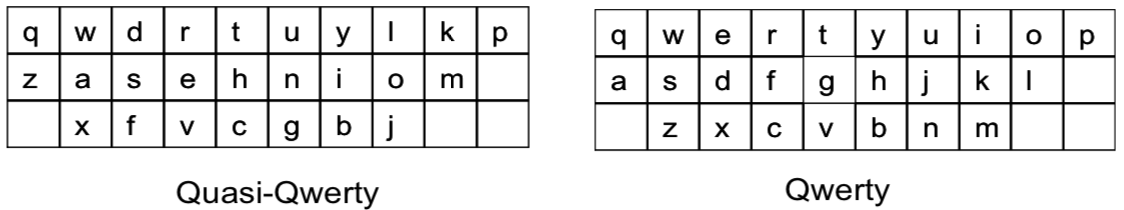
\includegraphics[width=0.8\textwidth]{Layout2010.png}
  \caption{New keyboard layout (left) from \citep{10.1145/1753326.1753367}}
  \label{fig:layout2010}
\end{figure}

Using the sum of Fitts’ law movement time between all pairs of letters along with the constraint on the QWERTY layout, the new layout was designed and shown in Figure \ref{fig:layout2010}. The predicted entry speed for Quasi-Qwerty keyboard was not as high as the freely optimized one, but higher than the conventional QWERTY keyboard. However, in the experiment, the initial entry time was shorter for the Quasi-Qwerty keyboard than the freely optimized one, which means novice users found it easier to transfer to this design. This paper reminded us that the performance was not the only criteria when designing a keyboard. Human factors such as the movivation to transfer to the new design should also be considered.

The reduced keyboard layout mentioned in \citet{10.1145/985921.986082} could not only applied to physical keyboard. With the development of tablet, a similar one-line keyboard layout was proposed by \citet{10.1145/2047196.2047257}, aiming for touch screen mobile devices with large screen, to maximize the displaying area for contents so that users did not have to swipe up and down constantly while typing. The new keyboard was only 39.8\% height of the native keyboard.

\begin{figure}[H]
  \centering
  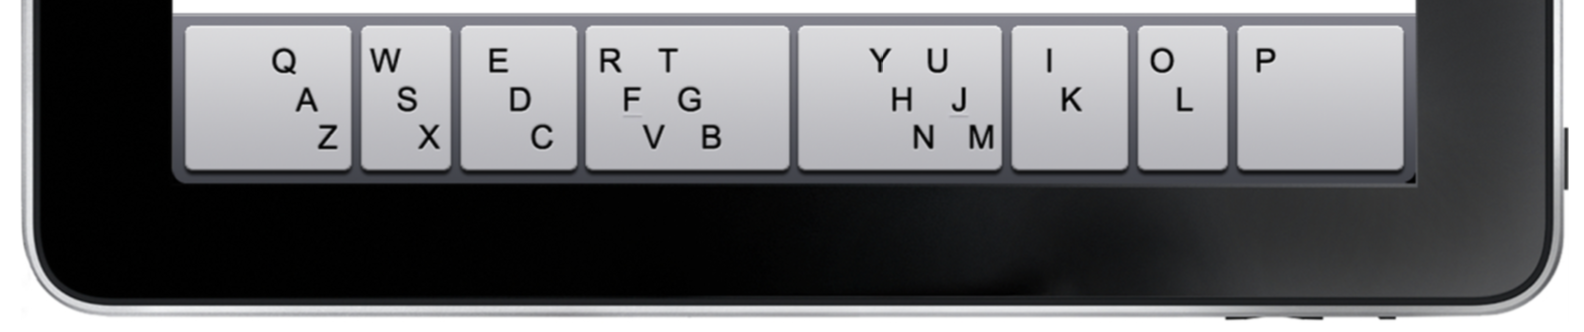
\includegraphics[width=0.8\textwidth]{Layout2011.png}
  \caption{New keyboard layout from \citep{10.1145/2047196.2047257}}
  \label{fig:layout2011}
\end{figure}

This design (Figure \ref{fig:layout2011}) also compressed the three-line QWERTY keyboard into one line. And based on the usage rate for each key, the keyboard further reduced (combined) some keys. The input process was close to the input on a T9 like keyboard. We typed the keys and selected the desired words predicted by the algorithm. The difference was that the "Enter", "Backspace" and word selection were done by gestures, which further reduced the number of keys. The experiemnt result showed participants could type at a rate of over 30 WPM after just five 20-minute typing sessions. And the predicted text entry speed was 68 wpm.

Above are three papers trying to improve the typing experience on mobile devices. Each of them had their own consideration: typing speed and error rate, users' motivation of switching and the size of the keyboard. When designing a new layout, these criteria can also be considered for the future researchers.

\subsection{Touch Screen Keyboard Layout Modification For Smaller Devices}

The smartwatch industry has been flourishing in the recent years. And with the development of mobile CPU, the functions of smartwatch went from simple calculation, digital time telling in the 2000s, to text messaging, sleep tracking, workout tracking in the 2010s. Although the speech recognition for text input on smartwatch is rather convenient now, sometimes out of privacy and other issues, we still want to choose to typing for text entry. It would be awkward to put the QWERTY keyboard directly on the smart watch since the screen size is too small to type. Therefore, new layouts for small touch screen devices were required.

One of the natural thoughts came up when tackling this problem was enlarge the keys. \citet{10.1145/2470654.2481387} proposed ZoomBoard, in which the keys were iteratively zoomed to a comfortable size to be seen.

\begin{figure}[H]
  \centering
  \includegraphics[width=0.8\textwidth]{ZoomBoard.png}
  \caption{New keyboard layout from \citep{10.1145/2470654.2481387}}
  \label{fig:zoomboard}
\end{figure}

Figure \ref{fig:zoomboard} above shows the working mechanism of the Zoomboard. In order to correctly detect which part of the keyboard and which specific area on the keyboard were selected, the authors  experimented with three zooming strategies. And they found that upon pressing the screen, the keyboard zoomed and leaving the target directly under the finger was the best approach. The ZoomBoard could be as tiny as the size of a US penny. The experiment found after the fianl trial, participants could achieve an average typing speed of 9.3 wpm, which was more than 100\% faster than directly using QWERTY keyboard on the screen. And the error rate was significantly lower as well.

Another approach to solve this problem was much the same as the one-line keyboard \citep{10.1145/2047196.2047257} mentioned above. If the size of the individual key was too small, just combine multiple keys together and enlarged the key size. \citet{6926662} brought out a keyboard for smart watch with six keys.

\begin{figure}[H]
  \centering
  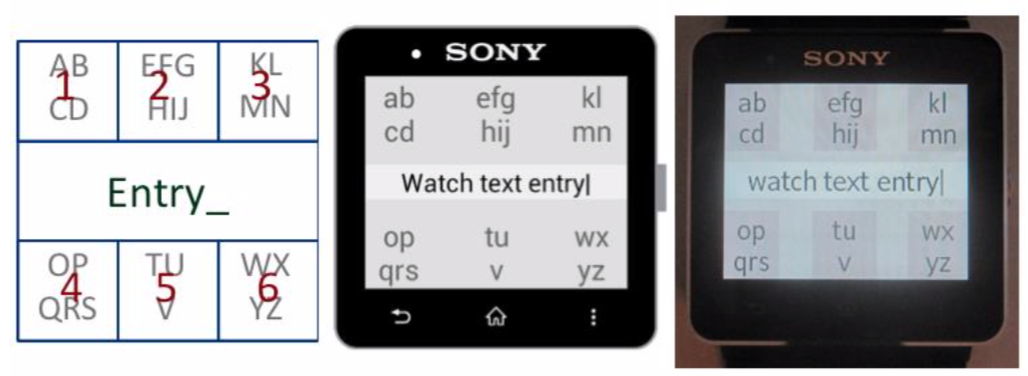
\includegraphics[width=0.8\textwidth]{Watch2014T9.png}
  \caption{New keyboard layout from \citep{6926662}}
  \label{fig:watch2014t9}
\end{figure}

Figure \ref{fig:watch2014t9} above shows the layout of the keyboard. When users pressed a key, the word with most probability based on the current character sequence was shown in the middle area of the screen. Then users could tap in the center screen to rotate through all the possible words. The backspace, numbers and capitalization were done by different swiping gestures on the screen. And the keyboard even supported adding accent marks by long pressing. The result indicated that the average typing speed was 8.1 wpm. It was not better than that of the ZoomBoard but this keyboard supported word suggestion, numbers and accent marks, which reduced the typing actions required and was more functional.

\citet{10.1145/2642918.2647354} outlined the Swipeboard for text entry on smartwatch. It leveraged users' spatial memory of a QWERTY keyboard, making it easy to learn, and it could even be operated under eyes-free condition.

\begin{figure}[H]
  \centering
  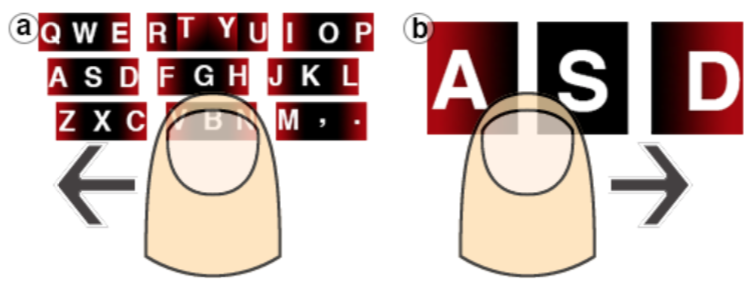
\includegraphics[width=0.8\textwidth]{SwipeBoard.png}
  \caption{New keyboard layout from \citep{10.1145/2642918.2647354}}
  \label{fig:swipeboard}
\end{figure}

Figure \ref{fig:swipeboard} shows the mechanism of SwipeBoard. The keyboard could be as small as 12$\times$12mm. Users used two swipes to select a character. In the first swipe, one of the nine regions where the character located was selected and in the second swipe, the character in the region was selected. The backspace, numbers and symbols were also toggled using gestures. Experiment showed that after 2 hours of training, participants could achive a typing speed of 19.58 wpm, which was reported 15\% faster than their baseline. The authors also mentioned the potential migration of this keyboard to eyewear, such as to Google Glasses.

\citet{10.1145/2702123.2702273} proposed SplitBoard, another text entry method on smartwatches. The QWERTY layout was divided into two sections in the SplitBoard, and the section could be switched using horizontal flick gestures (Figure \ref{fig:splitboard}). The keys were selected by a simple press. This approach was more straight-forward than the previous solutions. The backspace and space and functional keys(nums, caps, symbols) were shown directly instead of toggled using gestures.

\begin{figure}[H]
  \centering
  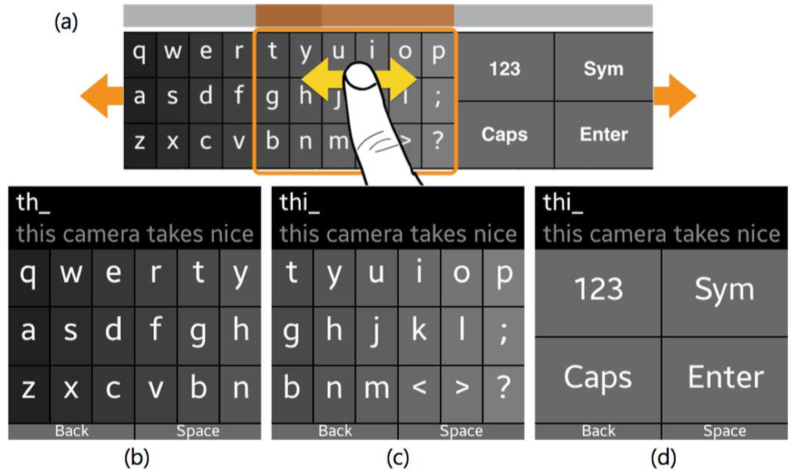
\includegraphics[width=0.8\textwidth]{SplitBoard.png}
  \caption{New keyboard layout from \citep{10.1145/2702123.2702273}}
  \label{fig:splitboard}
\end{figure}

The experiment result revealed that SplitBoard was faster than ZoomBoard and the native QWERTY keyboard on Samsung Galaxy Gear (29.3mm$\times$29.3mm touch screen) and the total error rate (TER) was the lowest among three keyboards and the uncorrected error rate (UER) was the same as QWERTY keyboard and lower than ZoomBoard.

\citet{10.1145/2858036.2858242} put forward WatchWriter (Figure \ref{fig:watchwriter}). Since it was difficult to modify the hardware, they moved their focus on the decoding algorithm. Instead of typing character by character, the strategy of WatchWriter was swipe typing. Users continuously swiped onto the approximate area of the keys in the word and relied on the algorithm to suggest the word. The space between words were automatically inserted and it also contained algorithm to avoid auto correct special words such as website URL. WatchWriter achieved a typing speed of 22-24 wpm with near zero error rate.

\begin{figure}[H]
\centering
\subfloat[WatchWriter from \citep{10.1145/2858036.2858242}\label{fig:watchwriter}]{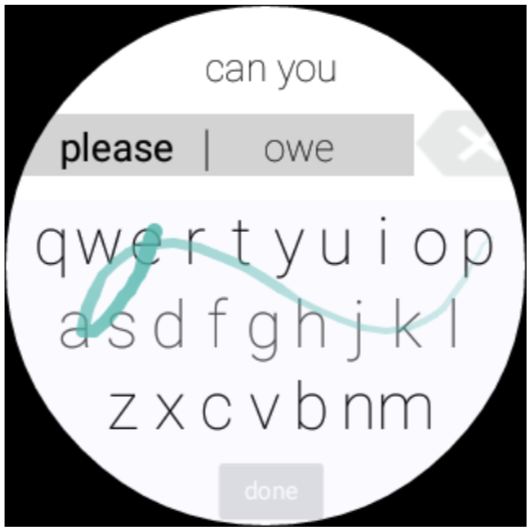
\includegraphics[width=0.2\textwidth]{WatchWriter.png}}\hfill
\subfloat[Invisiboard from \citep{10.1145/2935334.2935360}\label{fig:invisiboard}] {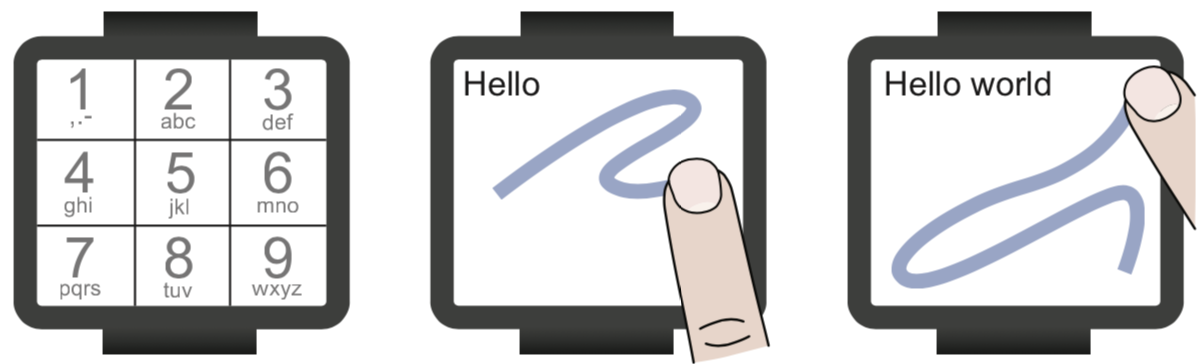
\includegraphics[width=0.7\textwidth]{Invisiboard.png}}\hfill
\caption{Comparison between WatchWriter(left) and Invisiboard(right)} \label{fig:watchcomparison}
\end{figure}

Finally, \citet{10.1145/2935334.2935360} proposed Invisiboard. It was a combination of the keyboard in \citet{6926662} and the WatchWriter \citep{10.1145/2858036.2858242}. Text input was done by swiping gestures, not on a QWERTY like keyboard but on a T9 like keyboard. Figure \ref{fig:watchcomparison} shows the difference between them. Subjects achieved an average of 10.6 wpm typing speed after 30 minutes practice and some participants demonstrated a speed of over 30 wpm.

To summarize, future researches on keyboard layout modification for small screen devices could refer to ideas mentioned in the above five papers. Each of the method had their own advantages and drawbacks. ZoomBoard could allow users to select a character in only one touch, but it did not have auto suggestions, and as mentioned by \citet{10.1145/2702123.2702273}, it would be slower than native QWERTY keyboard if the screen size was slightly larger. SwipeBoard required at least two press to select a character. SplitBoard cannot be applied on devices as small as the one used in ZoomBoard. And WatchWriter required the computing power of the smartwatch to perform real-time prediction. The combination of these ideas could potentially lead to a better design.

\subsection{Hiding The Touch Screen Keyboard}
A lot of effort has been devoted to maximize the displaying area on the touch screen. For instance \citet{10.1145/1851600.1851630} and \citet{10.1145/2212776.2223676} moved the physical keyboard to the back of the device, and \citet{10.1145/2047196.2047257} compressed the keyboard into one line. All those methods assume that a visible keyboard was necessary for typing. However, the standard keyboard layout has not been changed for decades and most of users have been using the QWERTY keyboard for at least several years. Some researchers have been thinking about hiding the keyboard completely, letting users type only with their own memory about the keys' position. Compleletely hiding the keyboard could free up a large portion of screen for content display.

\citet{10.1145/1978942.1979301} examined and compared the typing pattern under three conditions, when there was no visible keyboard and with/without error feedback and when there was visible keyboard and error feedback. The experiment assumed users type with ten fingers on a touch screen tablet, thus they could use their memory of touch typing experience on physical keyboard. The error feedback in the experiment was asterisks -- users could not tell what they type but they could know if they missed or made an extra press. The result indicated that after 5 practice sessions, and when there was no keyboard and no feedback, users could achieve 59 wpm typing speed if they assumed their input was correct, which was about 100\%faster than that on touch screen devices (30 wpm) and about the same as that on physical keyboard (60 wpm) \citep{10.1145/3173574.3174220}. With the feedback under the invisible keyboard condition, the typing pattern experienced a larger spread of hits per key comparing to the condition when the keyboard was visible, but still the classification accuracy was about 90\%. The result revealed that typing on a flat surface with no visble keyboard was possible. And some advice for invisible keyboard and algorithm design were given by the authors, such as the space bar should be shorter and taller; the key size should be larger and there should be a gap in the middle of the keyboard.

Based on this finding, \citet{10.1145/3173574.3174013} explored the possibility of typing with invisible keyboard on the mobile phone. The difference between typing on invisible keyboard on flat surface and mobile phone was that the latter used only two thumbs or an index finger, under which condition the knowledge about ten fingers muscle memory may not be used. The research found that users could utilize their memory of the layout of the QWERTY keyboard even with only one or two fingers typing. And with the modification on the decoding algorithm, an average speed of 37.9 wpm could be achieved after a few sessions of practice, making it undistinguishable from the typing speed on normal keyboard.

Those researches revealed that an invisible user interface was possible for mobile keyboards. It was a effective way to maximize the screen display area. To implement this design, several things should be modified comparing to the native keyboard, such as the key size, the curature of the keyboard and the decoding algorithm. In addition, since the keyboard was invisible, we should wisely deal with the components originally covered by the keyboard, avoiding conflicts between those components and the keyboard. And the workload should be further investigated by future research. After all, no one wants to switch to a keyboard that may make him/her distracted or exhausted.

\subsection{Utilizing Gestures}
The use of gestures has shown its own advantages on ultra-small screens, like WatchWriter \citep{10.1145/2858036.2858242} and Invisiboard \citep{10.1145/2935334.2935360}. Comparing with keyboards for desktop computers, keyboards on tablets and mobiles are relative small as well. Researches have been conducted to explore whether the use of gestures on these devices would improve the typing experience.

\citet{10.1145/642611.642630} designed \textit{SHARK} shorthand gesturing stylus keyboard. The design was based on two observations: (1) some characters in a word were connected in stylus keyboard, therefore swiping on them using gestures was faster than hitting the keys one by one; (2) users tended to remember the pattern of a word, that is, the trajectory of stylus movement from key to key, rather than individual key taps. Experiment showed after 45 to 50 minutes of practice session, subjects could reached a speed of 15 wpm. And most participants found it fun and even considered replacing physical typing from time to time. 15 wpm was not fast at all, as some of the optimized text entry methods on smartwatches like WatchWriter \citep{10.1145/2858036.2858242} could achieve 24 wpm. But considering the experiment was performed in 2003, at which time the devices were less optimized, it was a big step towards the application of gesture typing.

\citet{10.1145/1520340.1520380} proposed ShapeWriter, a gesture keyboard on iPhone. ShapeWriter was a stroke gesture-based text and command input method. Instead of tapping each individual letter, the user traces over all letters in a word sequentially on the touch screen keyboard. The difference between this text entry method and the ones in all other papers was that ShapeWriter was actaully put on AppStore. So the feedback could be directly reflected by the user comments. 454 (81.6\%) reviews was completely positive, and 12.5\% reviews was somewhat positive. Most of the positive reviews were about the performance of this new keyboard and wanted the keyboard to be applied system wide. Only 5.9\% reviews were completely negative, and most of them complained about their inadaptation. Overall, the gesture typing could be accepted by the public. And that is why Apple officially added this feature in iOS 13.

\begin{figure}[H]
  \centering
  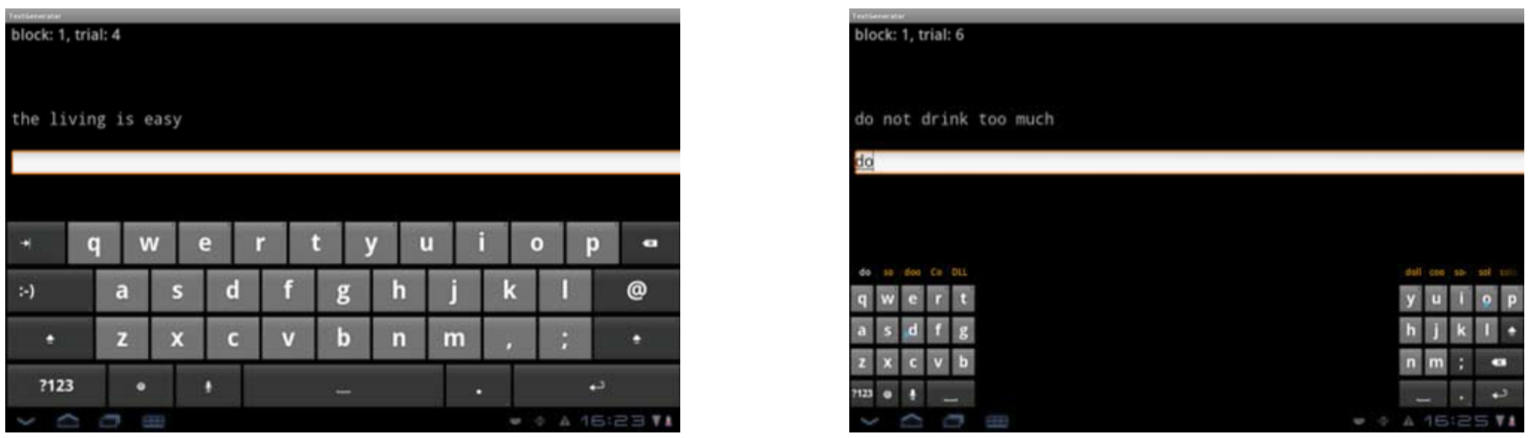
\includegraphics[width=0.8\textwidth]{Bimanual.png}
  \caption{Bimanual keyboard from \citep{10.1145/2380116.2380136}}
  \label{fig:bimanual}
\end{figure}

\citet{10.1145/2380116.2380136} proposed a bimanual gesture keyboard. For most gesture keyboards, the input was done by only one hand. However, most touch screen devices currently have the ability to multitouch and the size of the tablet is suitable for two hands performing gestures simultaneously. Researchers designed the algorithm to recognize multiple key strokes for the same word and suggested two approaches to detect the end of a word: finger-release, for which the release of both fingers indicated the end of a word, and space-required, for which the press of space button indicated the end of a word. Experiment showed that finger-released version of bimanual keyboard achieved about 85\% input speed of the conventional unimanual gesture keyboard. And the error rate was higher for finger-released bimanual (3.3\%) than unimanual (2.8\%). Space-released bimanual keyboard was not as good as the finger-released one. Although the bimanual keyboard was not as efficient as the unimanual keyboard, it takes only 25\% (landscape) and 47\% (portrait) space of the unimanual keyboard, and users expected about 50\% less key stroke length when typing. Figure \ref{fig:bimanual} shows the comparision between unimanual and bimanual gesture keyboards.

In conclusion, gesture keyboard is a proper way to balance the input performance and the keyboard size. Thus, it should be considered when trying to improve the overall user typing experience.

\subsection{Considering Postures}
Some users preferred to type with two thumbs on touch screen mobile devices and others preferred using index fingers. The typing pattern may be influenced by different postures and thus influence typing preformance and user experience. Researches have been performed to explore the relationship between typing postures and typing patterns.

\citet{twothumb2002} surveyed the the model of two-thumb text entry on physical keyboard on PDA, which is the earliest research about the typing posture on mobile devices. They predicted an upper bound of text entry rate of 60.74 wpm based on the linguistic and motor component of the interaction.

\begin{figure}[H]
\centering
\subfloat[Vertical Offset\label{fig:posturevertical}]{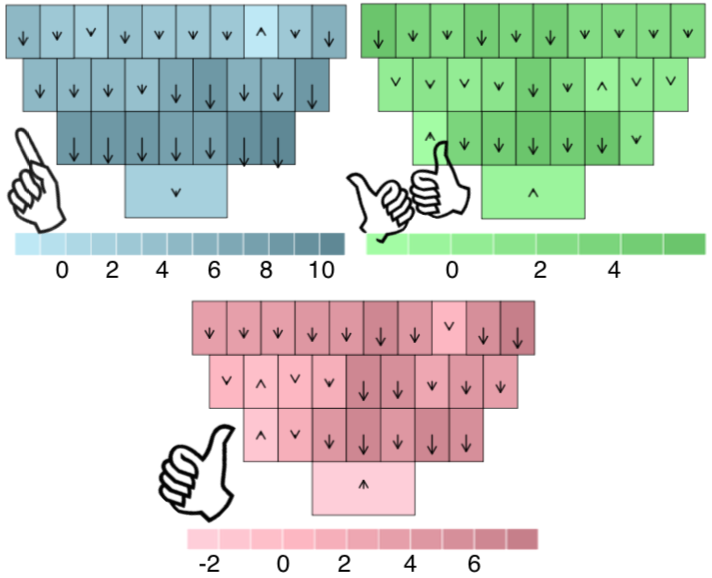
\includegraphics[width=0.5\textwidth]{Posture1.png}}\hfill
\subfloat[Horizontal Offset\label{fig:posturehorizontal}] {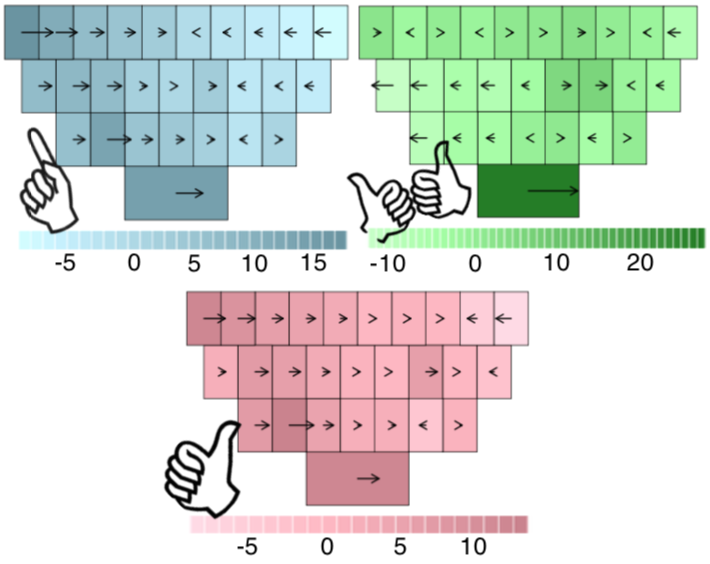
\includegraphics[width=0.5\textwidth]{Posture2.png}}\hfill
\caption{Postures VS Touch Points Offset from \citep{10.1145/2371574.2371612}} \label{fig:posture}
\end{figure}

\citet{10.1145/2371574.2371612} compared the touch behavior of different typing postures, namely, one finger, one thumb and two thumbs. They found that text entry with two thumbs was the fastest (50.03 wpm), one finger was far lower (36.34 wpm) and one thumb was the lowest (33.78 wpm). The error rate exhibited the same pattern as the entry rate: the higher the text entry rate, the higher the error rate. They also explored the touch points of all three postures. Vertically, touch points of all postures tend to be higher than the center of the key. And horizontally, touch points of one finger tend to be close to the center of the keyboard, that is, positive offset for keys on the left and negative offset for keys on the right; touch points of two thumbs tend to be close to the edge of the keyboard, that is, negative offset for keys on the left and positive offset for keys on the right; touch points of one thumb was similar to that of one finger but the pattern was not symmetric. Figure \ref{fig:posture} shows the typing pattern. Overall, all postures minimized their finger movement when typing. 

This research provided guidance for keyboard design when considering postures. The distribution and the decoding algorithm of the keyboard could be customized based on users' different typing postures.

ContextType \citep{10.1145/2470654.2481386} was a method using typing postures to improve the mobile touch screen text entry. Researchers first collected data for all four typing postures: using two thumbs, the left thumb, the right thumb, or the index finger. Then a touch pattern model was built based on that data and applied to the software keyboard. The keyboard would automatically detect one of the four typing postures based on information collected before while the user was typing and automatically switch to another algorithm if change was detected. Experiment showed the typing speed was not improved but the error rate was lowered by 20.6\% for all four postures by the application of ContextType. This experiment confirmed the theory proposed in \citet{10.1145/2371574.2371612} and proved the adaptation of posture context could indeed make some improvement to the typing experience.

\subsection{Algorithm Enhancement}
The improvement in algorithm could significantly improve the typing experience. And usually, a new algorithm was combined with some other technologies or research findings, such as Invisiboard \citep{10.1145/2935334.2935360} combined a new reduced keyboard with new decoding algorithm; ContextType \citep{10.1145/2470654.2481386} combined the keyboard with a posture detection algorithm, etc. In this subsection, several approaches concentrating on the algorithm design to enhance typing were introduced.

\citet{10.1145/1357054.1357147} designed a system -- Automatic Whiteout++ to detect and correct errors made by typists on physical mini-QWERTY keyboard. In their previous system Automatic Whiteout, the algorithm could already detect typos like row substitution error (e.g. cat to cay), key repeat error (e.g. cat to caat), roll-on insertion error (e.g. cat to cart) and roll-off insertion error (e.g. cat to catr). In this new system, bi-letter and tri-letter frequency were introduced to help with error detection. And a decision tree was used to decide whether or not a word was a typo. Experiment showed the new system could detect and correct up to 32.37\% of errors. One drawback of this system was that it did not use the dictionary information, maybe it was constrained by the computing power for mobile devices at that time, combining of which may lead to a better result.

\citet{10.1145/2702123.2702135} proposed VelociTap, a pure keyboard decoder that supported a sentence-based text entry approach. The decoder used a probabilistic keyboard model, a character language model, and a word language model. The algorithm was designed by adding the keyboard model log probability to the language model log probability multiplied by a scaling factor. And the result was used to search for the top 50 probable hypotheses. The system was trained with billions of words from blogs and social media. The experiment result indicated the system could achieve a similar text entry speed as Google keyboard but a much lower error rate.

In addition to the decoder algorithm improvement, key resizing and adaptation algorithms were popular and effective as well. \citet{10.1145/2207676.2208520} proposed an algorithm based on touch location, touch area, finger movement, previous key press and the position of hand and arm. The keys with the top probability for the next candidate were enlarged or moved slightly to a preferred position. Result showed that while remaining a low error rate, the adapted keyboard outperformed the conventional one. 

\begin{figure}[H]
  \centering
  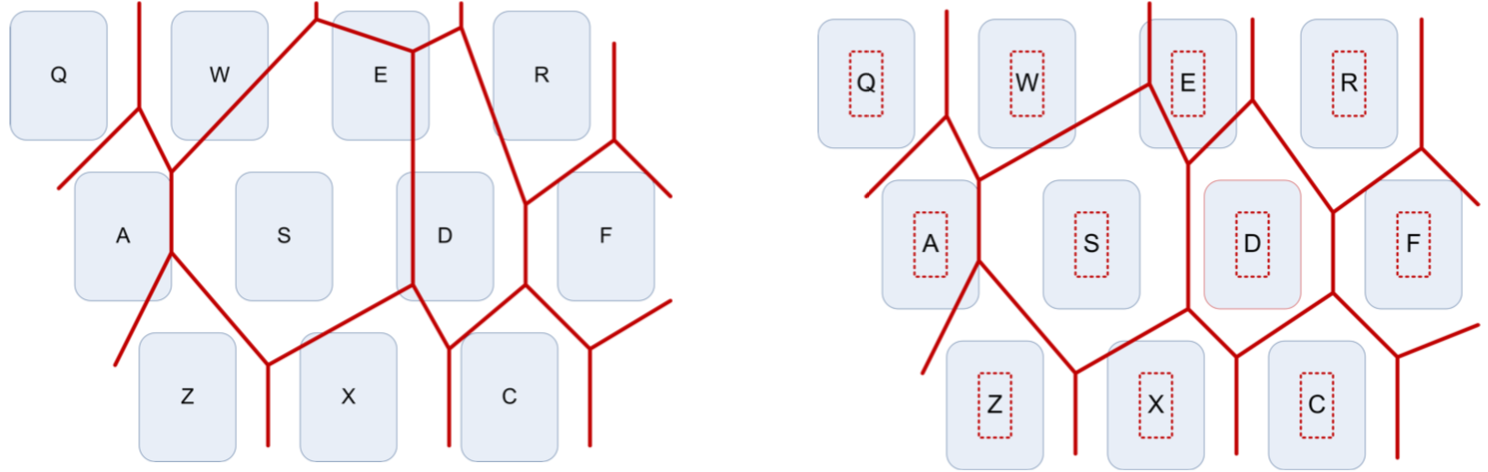
\includegraphics[width=0.8\textwidth]{Usability.png}
  \caption{Keyboard adaptation \citep{10.1145/1719970.1719986}, left: unconstrained, right: constrained}
  \label{fig:usability}
\end{figure}

Furthermore, \citet{10.1145/1719970.1719986} did a usability research on auto adaptive keyboards, the result showed those keyboards could lower the error rate. However, the authors also adviced the designers to add constraints to the adaptation algorithm (Figure \ref{fig:usability}(right)), since a too extreme algorithm would make it impossible to tap some keys, as it is shown in Figure \ref{fig:usability}(left).

Finally, \citet{10.1145/2470654.2481384} combined the posture adaptation and keyboard layout adaptation together. Using a hierarchical spatial backoff model with submodels of different levels of complexity, they reduced the language-model-independent error rate by 13.2\%.

\subsection{Text Entry User Experience Improvement: Conclusion}
In this section, potential methods to improve the user experience when typing were summarized. Shrinking the keyboard, moving the keyboard to the back or making keyboard invisible could be used to maximizing display area. Modifying keyboard layout, adding physical feedback, and other methods related to postures or gestures could be used to improve the typing speed or lower the error rate or both. And designing a new decoding/adaptive algorithm could be beneficial in all aspects. When designing a highly efficient and user attracting keyboard on mobile devices, the factors in this section should be considered.

\newpage
\bibliographystyle{apalike}
\bibliography{references}

\end{document}
